\documentclass[a4paper,oneside,11pt]{report}
\usepackage{cite}
\usepackage[utf8]{inputenc}
\usepackage[francais]{babel}
\usepackage[nodisplayskipstretch]{setspace} 
\usepackage[dvips,a4paper]{geometry}
\usepackage[hang,small,bf]{caption}
\usepackage{caption}
\usepackage{graphicx}
\usepackage{float}

\geometry{lmargin=2.5cm,rmargin=2.5cm,vmargin=4cm}
\setlength{\parindent}{1cm}
\renewcommand\thesection{\arabic{section}}


\begin{document}

\pagestyle{plain}
\setstretch{1.2}
\vspace{2ex}%
\begin{center}
\bfseries\Huge{L'eXtreme Programming}
\end{center}
\vspace{3ex}%

Le but de ce papier est de présenter dans un premier temps les idées de base de la programmation extrême (XP en anglais) de même que l'origine du nom puis dans un second temps les valeurs et pratiques associées à l'XP.

Au début des années 2000, l'XP était de loin la méthode agile la plus populaire ainsi que la plus discutée. Aujourd'hui l'emploi du terme XP semble moins prononcé dans la littérature, néanmoins les principes fondamentaux de l'XP forment les bases de la plupart des méthodes agiles modernes (SCRUM, KABAN...). L'XP est basée sur un ensemble de concepts de génie logiciels utilisés depuis longtemps dans l'industrie (Taylorisme), mais la version originale a été publiée en 1999 dans le livre de Kent Beck "Extreme Programming Explained: Embrace Change". Une évolution lui sera apporté en 2004 dans une version baptisée XP2 : certaines pratiques y seront modifiées ainsi que d'autres rendues plus précises. \\

\section{Les Valeurs}
L'XP dans sa totalité (en terme de règles et de pratiques) est basé sur cinq idées fondamentales appelées "Valeurs" :
\begin{itemize}
\item La Communication
\item La Simplicité
\item Le "feed-back"
\item Le Courage
\item Le Respect
\end{itemize}

Ces valeurs donnent ainsi le ton à une discipline collective générale.

\subsubsection{La communication}

La plupart des problèmes inhérents aux projets sont liés à une communication de mauvaise qualité voir meme complètement inexistante. Exemple : mauvaise coordination des déçisions, manque d'informations sur les changements décidés, 
De ce fait XP impose la communication comme règle d'or : elle doit être fréquente, rapide et efficace. De plus certaines pratiques de l'XP imposent la communication : 
D'un point de vue générale par le biais de réunions hebdomadaires inter-équipe
lors de la programmation en binome : A écrit du code, B corrige et analyse en temps réel. 
L'utilisation d'un espace de travail commun,  sorties fréquentes de releases (communication vers le client).


\subsubsection{La simplicité}

Les solutions simples possèdent de nombreux avantages : elles sont simples à designer, simple à implémenter, tester, débuger, expliquer, changer....  Celà est vrai autant pour les produits que pour les processus. De ce fait L'XP choisit de toujours employer la solution la plus simple au jour J sans en rechercher une  plus complexe dans l'espoir d'une utilité future. Leur slogan : "You Ain't Gonna Need It" (YAGNI).


\subsubsection{Feedback (retour)}

Il est extrêmement utile pour n'importe quel projet d'avoir des retours rapides et fréquents sur les actions menées jusqu'alors. Cela évite ainsi de partir trop longtemps dans une "mauvaise direction". Cela permet de répondre rapidement aux questions du type   : Est-ce que ce morceau de code est correct ? S'articule -t'il correctement avec le reste du projet ? Le système global est il utile ? 
Ainsi, l'XP intègre le feedback le plus souvent possible par le biais de ces pratiques exemple :
Test de chaque partie de code
Intégration continue
Itération courtes
releases fréquentes



\subsubsection{Le courage}

Les trois valeurs enoncées précédemment requièrent du courage, englobant la prise initiative et une forte implication personelle. L'échec n'est pas une fin en soi mais un moteur de progrès.

\subsubsection{Le Respect}

La cohésion et l'existence même de l'XP  découlent directement du respect entre les différents acteurs du projet. Le blâme est inutile. Un coach fera office de médiateur.




\section{Les pratiques}


\begin{figure}[!h]
\begin{center}	
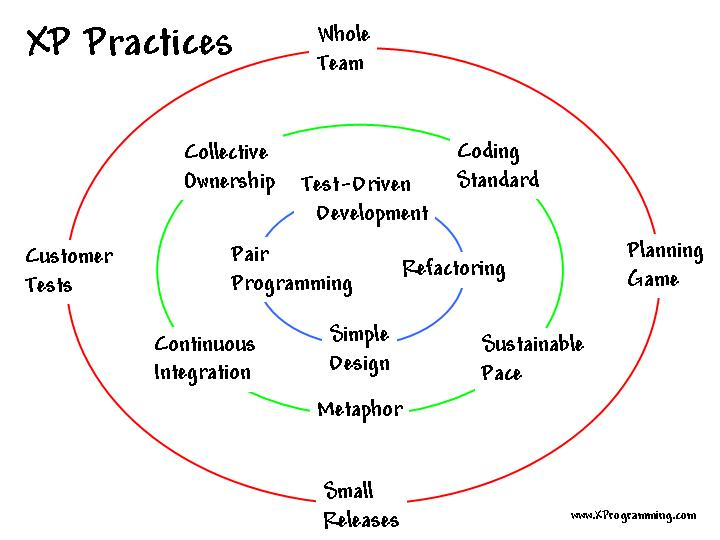
\includegraphics[height=7.013cm,width=8.53cm]{circles.eps}
\caption{\label{fig1}Les pratiques de l'XP} 
\end{center}
\end{figure}


La méthode XP est constituée d'un ensemble de pratiques. Ces pratiques restent néanmoins flexibles dans leur applicabilité, néanmoins chacune d'elle devra être présente pour parler d'un vrai processus XP. Cependant, dans la pratique il arrive souvent que chacune d'elle ne soit pas utilisée. Choisir uniquement sa préférée ne fait pas partie d'XP ! Elles se renforcent mutuellement. Naturellement un même acteur sera affecté à de multiples pratiques.\\

Ci-dessous la liste des pratiques de XP2 :

\begin{itemize}
\item Sit Together : toute l'équipe travaille idéalement dans un espace de travail commun, cela favorise la communication informelle.
\item  Whole Team : L'équipe doit être complète et équilibrée, toutes les compétences doivent y être représentées (developpeurs, coach,  représentant client, ...)
\item Informative Workspace : Toute la structure du projet au temps $t$ doit être affichée dans l'espace de travail commun.
\item Energized Work : Chaque membre de l'équipe doit être motivé et s'impliquer personnellement dans le projet. L'ambiance doit être bonne, les pauses suffisantes et les heures supplémentaires sont proscrites.
\item Pair Programming : Chaque partie de code est développée en binôme sur une même machine. Cela permet de corriger les erreurs rapidement, d'apprendre de l'autre et d'avoir une meilleure expertise.
\item User Stories : Chaque exigence est traduite sous forme textuelle condensée et explicite.
\item Weekly Cycle : Le projet global est découpé en plusieurs parties appelées itération. Une itération représente un travail réalisable en une à deux semaines pour toute l'équipe et est composés d'une à plusieurs Stories. Elle constitue la plus petite unité temporelle du projet.
\item Quarterly Cycle : Ce cycle correspond à la validation du projet via release. Il est souhaitable d'en obtenir en pratique 4 par an.
\item Slack : Les developpeurs doivent consacrer une petite partie de leur temps de travail sur autre chose que le projet.
\item Ten-Minute Build : La compilation et l'exécution du système ne doit pas prendre plus de 10 min.
\item Continuous Integration : Chaque developpeur verifie plusieurs fois dans la journée la compatibilité de son travail avec le reste du code. Afin de faciliter cette pratique, des processus automatiques de vérification sont mis en place en background. Cela est très utile pour le bug-tracking.
\item Test-First Programming : Un test propre est mis en place dès le début de l'écriture d'un code. Il permettra au fur et à mesure de tester la validité des différentes parties implémentées.
\item Incremental Design : L'architecture est complétée étape par étape en parallèle du code. L'architecture globale n'est pas fixée à l'avance, les re-factorisations de code sont fréquentes.
\end{itemize}




\section{Résultats}

Plus de 90\% des projets ont été considérés comme réussis, et la moitié d'entre eux utilisaient XP pour la première fois. 100\% des utilisateurs souhaitent à nouveau utiliser cette technique.


\section{Critiques}

Outre les difficultés de mise en place des différentes pratiques liées a XP, plusieurs critiques ont été émises à son encontre. Ces critiques reposent sur le fait que l'XP théorique n'est applicable que dans de rares situations "utopiques". De plus, les compétences requises pour les membres de l'équipe sont généralement bien au dessus du niveau moyen et l'absence de documentation requiert une stabilité de l'équipe importante. En effet si l'un des membres venait à quitter le projet, son remplacement serait difficile et le projet en serait fortement impacté. De la même manière, la valeur de "simplicité" imposée par l'XP est rapidement mise à mal dans bon nombre de projets où l'architecture requiert une certaine complexité. 
D'un point de vue applicabilité, il a été montré que l'XP s'intègre préférentiellement sur des équipes à effectifs restreints ($<20$). Au delà, la méthode peut représenter un goulot d'étranglement et donc un frein à la productivité. Enfin, il est évident que sur des projets nécéssitant un temps de compilation long (\~ heure), XP n'est pas applicable


\section{Ressources}

\begin{itemize}
\item Kent Beck - Extreme Programming Explained: Embrace Change - 2nd Edition
\item http://www.agilealliance.com
\item http://www.xprogramming.com
\item http://c2.com/cgi/wiki?ExtremeProgrammingRoadmap
 \end{itemize}


\end{document}
